\documentclass{article}[12pt]
\usepackage[T1]{fontenc}
\usepackage[polish]{babel}
\usepackage[utf8]{inputenc}
\usepackage{graphicx}
\usepackage[table]{xcolor}
\usepackage{enumitem}
\usepackage{tabularx}



\title{Doskonała Praca Zespołowa esej}
\author{Krzysztof Rudnicki, 307585}

\begin{document}
\definecolor{lightgreen}{rgb}{0.9, 1, 0.9}
\definecolor{lightred}{rgb}{1, 0.9, 0.9}
\maketitle
\paragraph{Wstęp}
W ramach tego eseju opiszę działanie zespołu zajmującego się zarządzaniem Kołem Naukowym Twórców Gier Polygon (dalej KNTG Polygon lub Polygon), największym studenckim kołem twórców gier w Polsce, którego byłem przez rok wiceprezesem i przez rok prezesem.
\paragraph{Zespół}
KNTG Polygon jest zarządzany przez dwie grupy w hierarchii: niższą i liczniejszą, tak zwanych „magów”. oraz wyższą i mniej liczną, tak zwaną „kapitułą”, istnieje również specjalna grupa „emerytowanych” magów oraz członków kapituły - valhalla, pełniąca właściwie tylko funkcję doradczą średnio na Polygonie jest aktywnych około 20-25 magów oraz 5-7 członków kapituły
\paragraph{Role}
\begin{itemize}
\item Socjal Media - Ta osoba zajmuje się tworzeniem treści na media społecznościowe koła - facebook, discord, twitter itp.
\item „Ogarniacz” w dniu wykładu - co tydzień w środę, koło spotyka się na wykładzie, ta osoba jest odpowiedzialna za zdobycie karty do sali, przygotowanie sprzętu do prezentacji oraz zapowiadanie kolejnych wykładowców
\item Rezerwacja barów - Po wykładach Polygon udaje się na integrację w liczbie około 30-50 osób, zadaniem tej osoby jest znalezienie i zarezerwowanie baru na tyle osób
\item Załatwianie wykładów - Kontaktuje się z wykładowcami, szuka potencjalnych wykładowców, ustala terminy wykładów
\item Nadzór projektów mentorskich - Polygon organizuje projekty gdzie w ciągu jednego semestru w grupie losowych osób tworzy się grę, ta osoba zajmuje się przydzielaniem osób do grup i odpowiadaniem na ich potrzeby
\item Wolontariusz - Koło organizuje Game Jamy - imprezy podczas których w ciągu 1-3 dni tworzy się grę, podstawą udanej organizacji jest praca wolontariuszy, przenoszenie rzeczy z miejsca na miejsce, sprzątanie, rozdawanie koszulek, pilnowanie wejśc i reagowanie na potrzeby uczestników
\item Organizator - Zajmuje się przydzielaniem i nadzorowaniem wolontariuszy
\item Prezes - Najważniesza osoba w kole, zajmuje się nadzorowaniem całego koła i kontaktami z uczelnią
\end{itemize}
\begin{figure}[h]
\caption{Uproszczona struktura Polygonu}
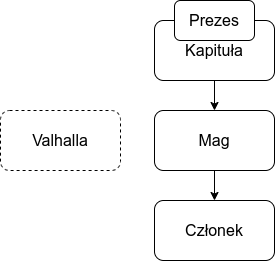
\includegraphics[width=\textwidth]{polygon_org.drawio.png}
\end{figure}
\paragraph{Struktura}
Pomimo podziału na magów, kapitułę i prezesa, struktura Polygonu jest bardzo płaska, każdy, również zwykły członek może wyjść z dowolną propozycją i bardzo często może ją od razu realizować, maksymalizuje to kreatywność, kosztem produktywności
\paragraph{Rozwój zespołu} 
Zespół magów i kapituły jest już rozwinięty i nowi członkowie dołączają do niego poprzez integrację z obecnymi magami i członkami kapituły, pozwala to na bardzo naturalne integrowanie zamiast tworzenia zupełnie nowego zespołu co semestr.
\paragraph{Cel}
Celem koła jest jego rozwój na wszystkich płaszczyznach, tworzenia większych wydarzeń, zapraszania bardziej prestiżowych wykładowców, zbierania więcej ludzi na wykłady, tworzenie lepszych projektów mentorskich, konkretny plan na dany semestr ustala Kapituła. 
\paragraph{Normy zespołowe}
Członkowie Polygonu ubierają się w lużny sposób, typowy dla branży programistycznej, nie ma narzuconego stylu ubierania się, komunikacja odbywa się na równej, przyjacielskiej zasadzie (domyślnie przechodzi się na „Ty”), unikalną cechą Polygonu jest posługiwanie się przede wszystkim pseudonimami (podobnymi do "nicków" z gier), jedyną narzuconą regułą jest właśnie potrzeba posiadania pseudonimu.
\paragraph{Integracja}
Co tydzień w środę po wykładzie następuje integracja nazywana „Piwem”, pomimo swojej nazwy można w niej uczestniczyć również nie pijąc piwa, przez wielu uczestników uważana za najważniejszą część spotkania, niektórzy chodzą tylko na piwo, poza tym Polygon organizuje również ogniska i game jamy. W obrębie kapituły oraz magów organizuje się również regularne spotkania
\begin{table}[h]
\caption{Porównanie mocnych i słabych stron Polygonu}
\centering
\begin{tabularx}{\textwidth}{|X|X|}
\hline
\cellcolor{lightgreen}\textbf{Mocne} & \cellcolor{lightred}\textbf{Słabe} \\ \hline
\begin{itemize}[leftmargin=*]
\item Brak konkurencji wewnątrz zespołu
\item Pozycja lidera - Prezesa
\item Szczera komunikacja
\item Dostęp do informacji
\item Szacunek
\item Przyjazna atmosfera
\item Dobre normy zespołowe
\item Dobre, sprawdzone metody integracji
\end{itemize} & 
\begin{itemize}[leftmargin=*]
\item Często mało konkretne cele
\item Często brak jasności w podziale ról
\item Brak jakichkolwiek kosztów wejścia
\item Pełny wolontariat, często prowadzący do wyboru innych priorytetów przez członków zespołu
\item Powolna wymiana na średnim szczeblu (magów)
\item Brak zastosowania jakichkolwiek metod heurestycznych
\item Brak badania ról zadaniowych poszczególnych członków
\end{itemize} \\ \hline
\end{tabularx}
\label{table:comparison}
\end{table}

\end{document}